%!TEX root = Thesis.tex

\chapter{Semantic networks}
\label{chap:SemanticNetworks}

In order to reason about the polarity of the selected subject in the review text, a understanding of the domain of the review is needed.  For this purpose the concept of \emph{semantic networks} is introduced. Formally it is defined follows:
\begin{definition}
a semantic network is a quadruple $(L,S,R,M)$ where:\\[-2em]
  \begin{itemize} %[labelindent=2em,labelwidth=0em,itemindent=0em,leftmargin=2em]
    \item $L$ is the set of lexical units recognized by the network.
    \item $S$ is the set of \emph{semantic concepts} in the network.
    \item $R$ is a set of binary relations on $S$ where the relation $r \in R$ describes links\\ between semantic concepts, i.e.\ $r \subset S \times S$. 
    \item $M$ is a mapping from lexical units to a set of semantic entities that the lexical\\ unit can entail, i.e.\ $M: L \to \mathcal{P}(S)$.
  \end{itemize}
  \label{def:SemanticNetwork}
\end{definition}

Notice that $S$ and $R$ constitutes a set of graphs, i.e.\ for each relation $r \in R$ the graph~$(S,r)$. The graph is undirected if $r$ is \emph{symmetric}, and directed if $r$ is \emph{asymmetric}.

\begin{figure}[ht]
  \center
  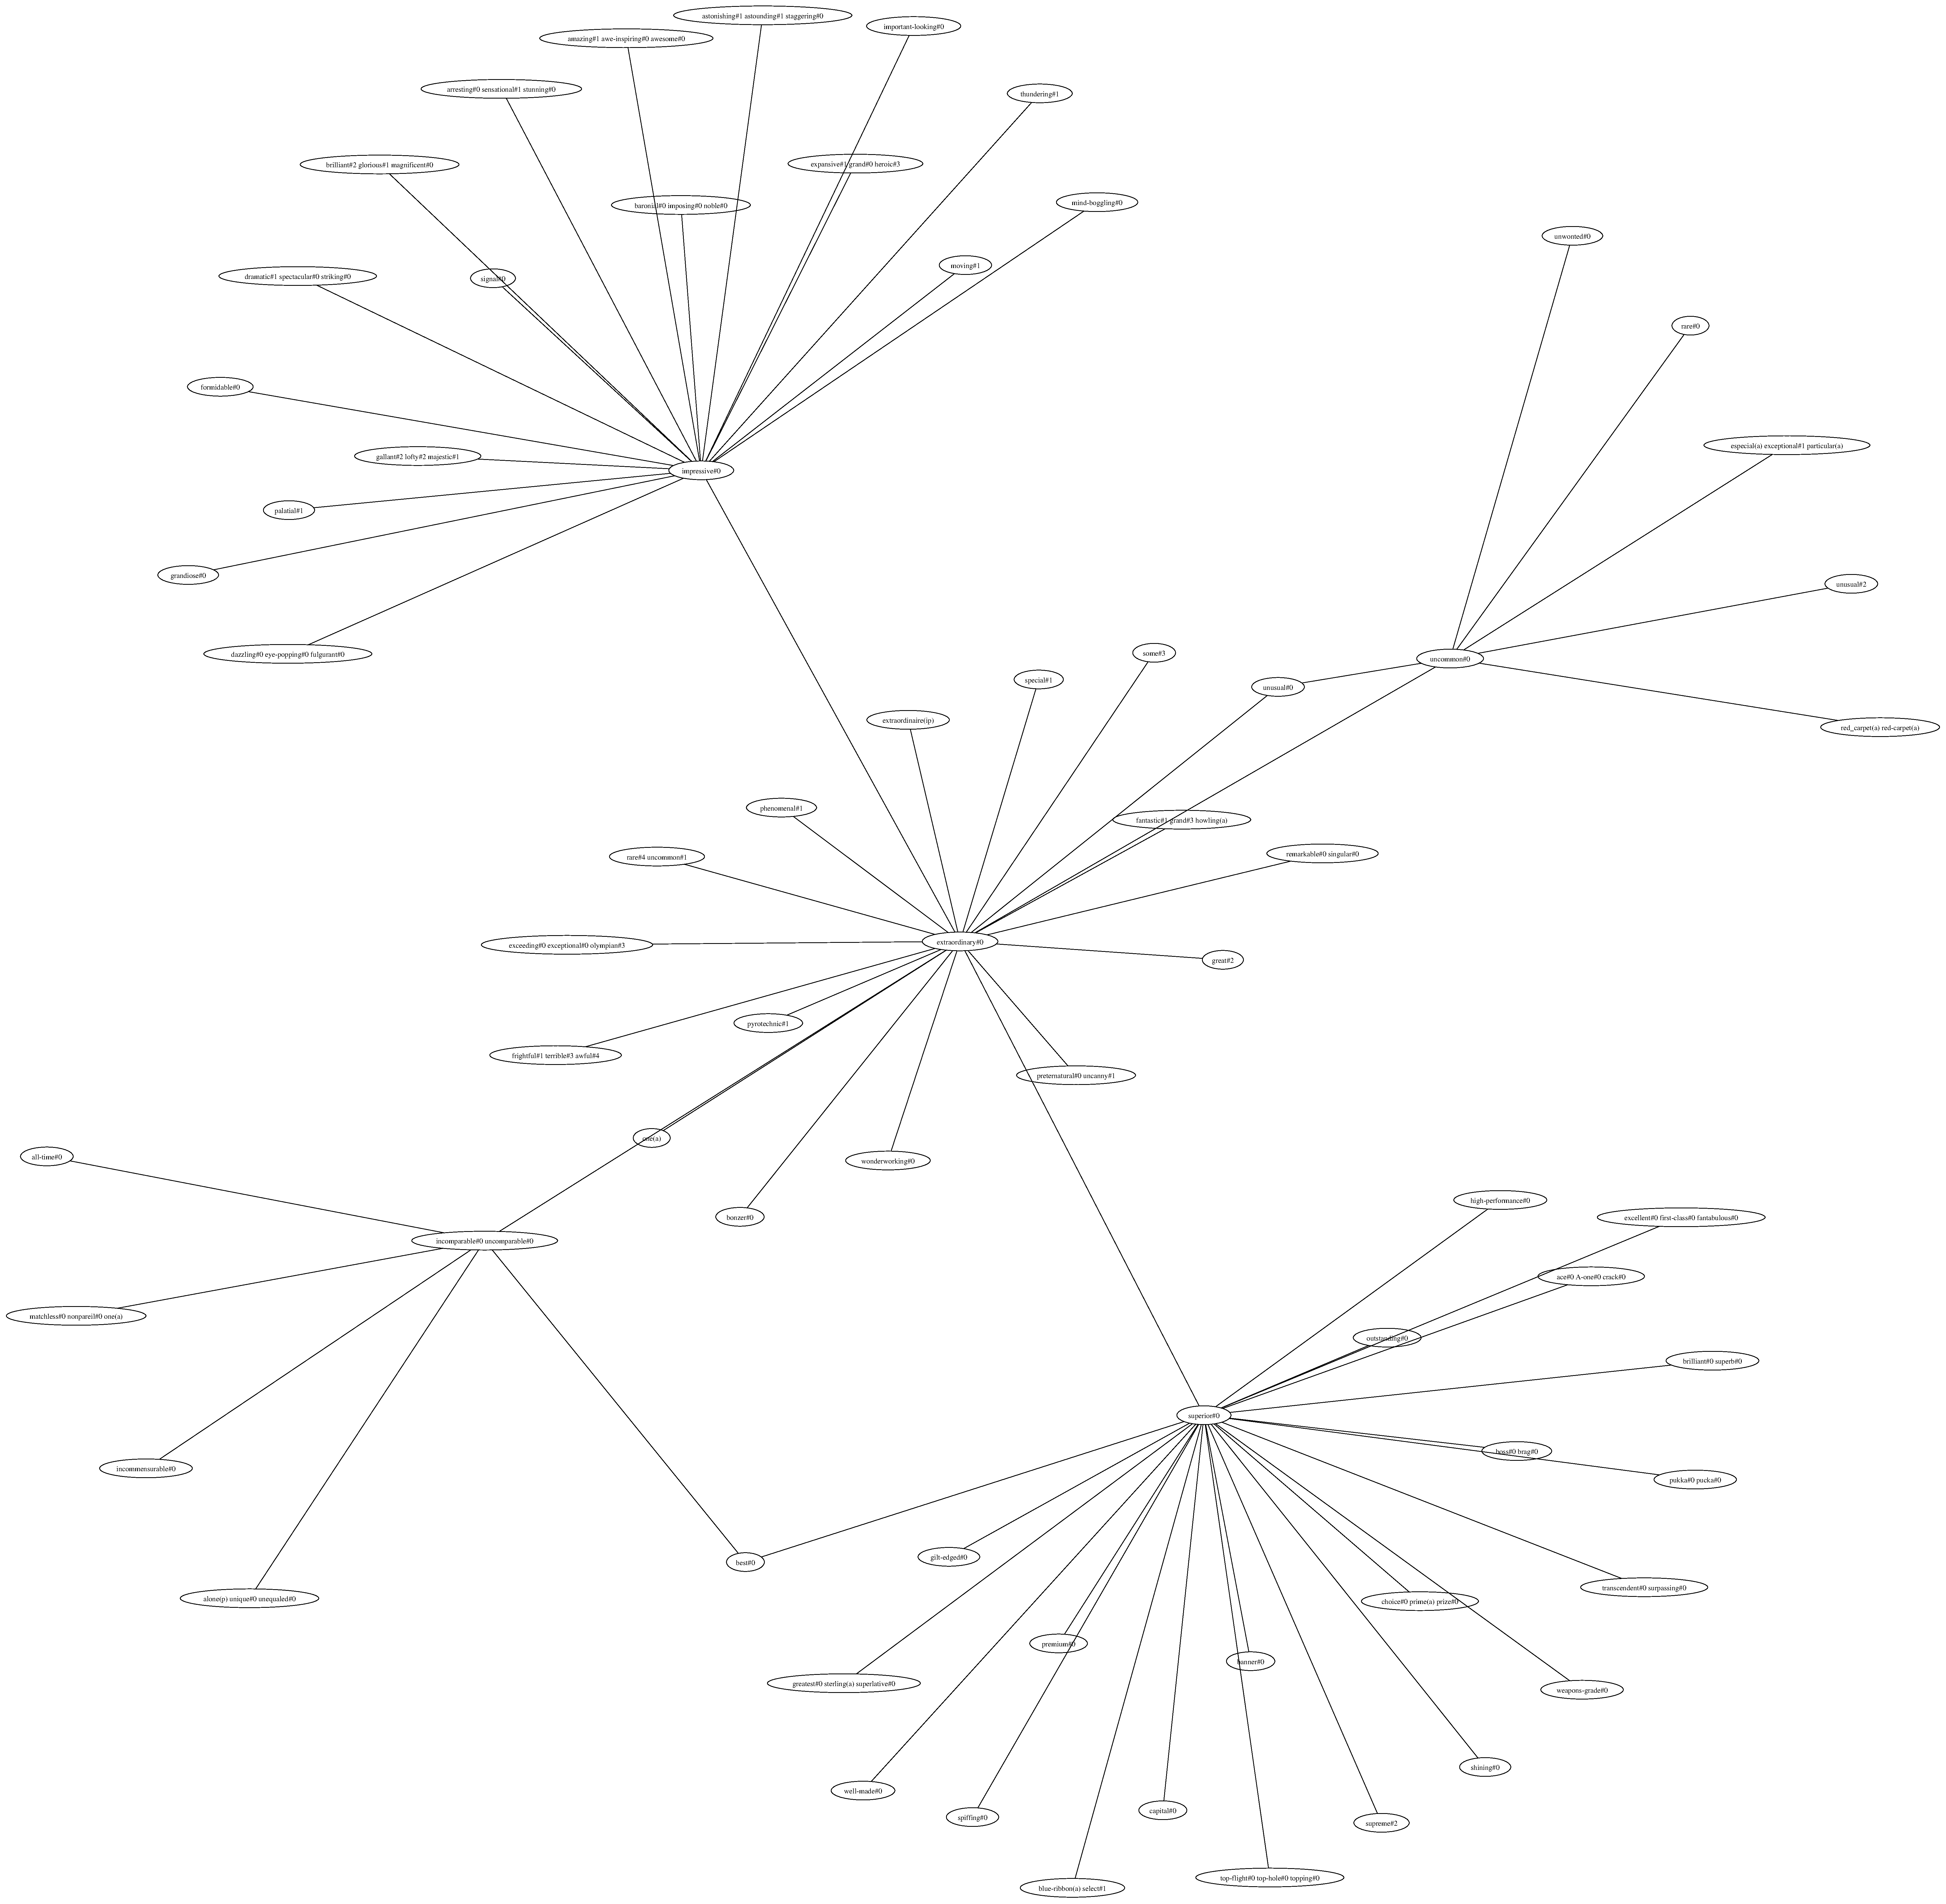
\includegraphics[scale=.4]{Figures/Exceptional}
\end{figure}

\cite[p. 453-456, 468, 471]{ai}

An illustrative example of such a graph, denoting a relation in a tiny semantic network of adjective concepts is given in figure X. The relation depictured . 
transitivity...


We have no way of detecting different semantic ambiguity, since we have no knowledge bade ... therefore we shall restrict our-self to 